\documentclass[gr-notes.tex]{subfiles}

\begin{document}

\setcounter{chapter}{4}

\chapter{Preface to Curvature}

\setcounter{section}{7}

\section{Exercises}

\textbf{1}

(a)
Repeat the argument leading to Equation 5.1, but this time assume that only a fraction $\epsilon < 1$ of the mass's kinetic energy is converted into a photon.

If only a fraction $\epsilon$ of the energy is converted into a photon, then it will start with an energy of $\epsilon (m + mgh + \order{\boldsymbol{v}^4}$, but once it reaches the top it should have an energy of $\epsilon m$, as it loses the component due to gravitational potential energy. Thus
%
\begin{displaymath}
  \frac{E'}{E} =
  \frac{\epsilon m}{\epsilon (m + mgh + \order{\boldsymbol{v}^4)}} =
  \frac{m}{m + mgh + \order{\boldsymbol{v}^4}} =
  1 - gh + \order{\boldsymbol{v}^4}
\end{displaymath}

(b)
Assume Equation 5.1 does not hold. Devise a perpetual motion device.

If we assume that the photon does not return to an energy $m$ once it reaches the top, but instead has an energy $m' > m$, then we could create the perpetual motion device shown in Figure \ref{fig:ch5-problem-1b}. A black box consumes the photon with energy $m'$, and splits it into a new object of mass $m$, and a photon of energy $m' - m$. The object repeats the action of the original falling mass, creating an infinite loop.

\begin{figure}[b]
  \centering
  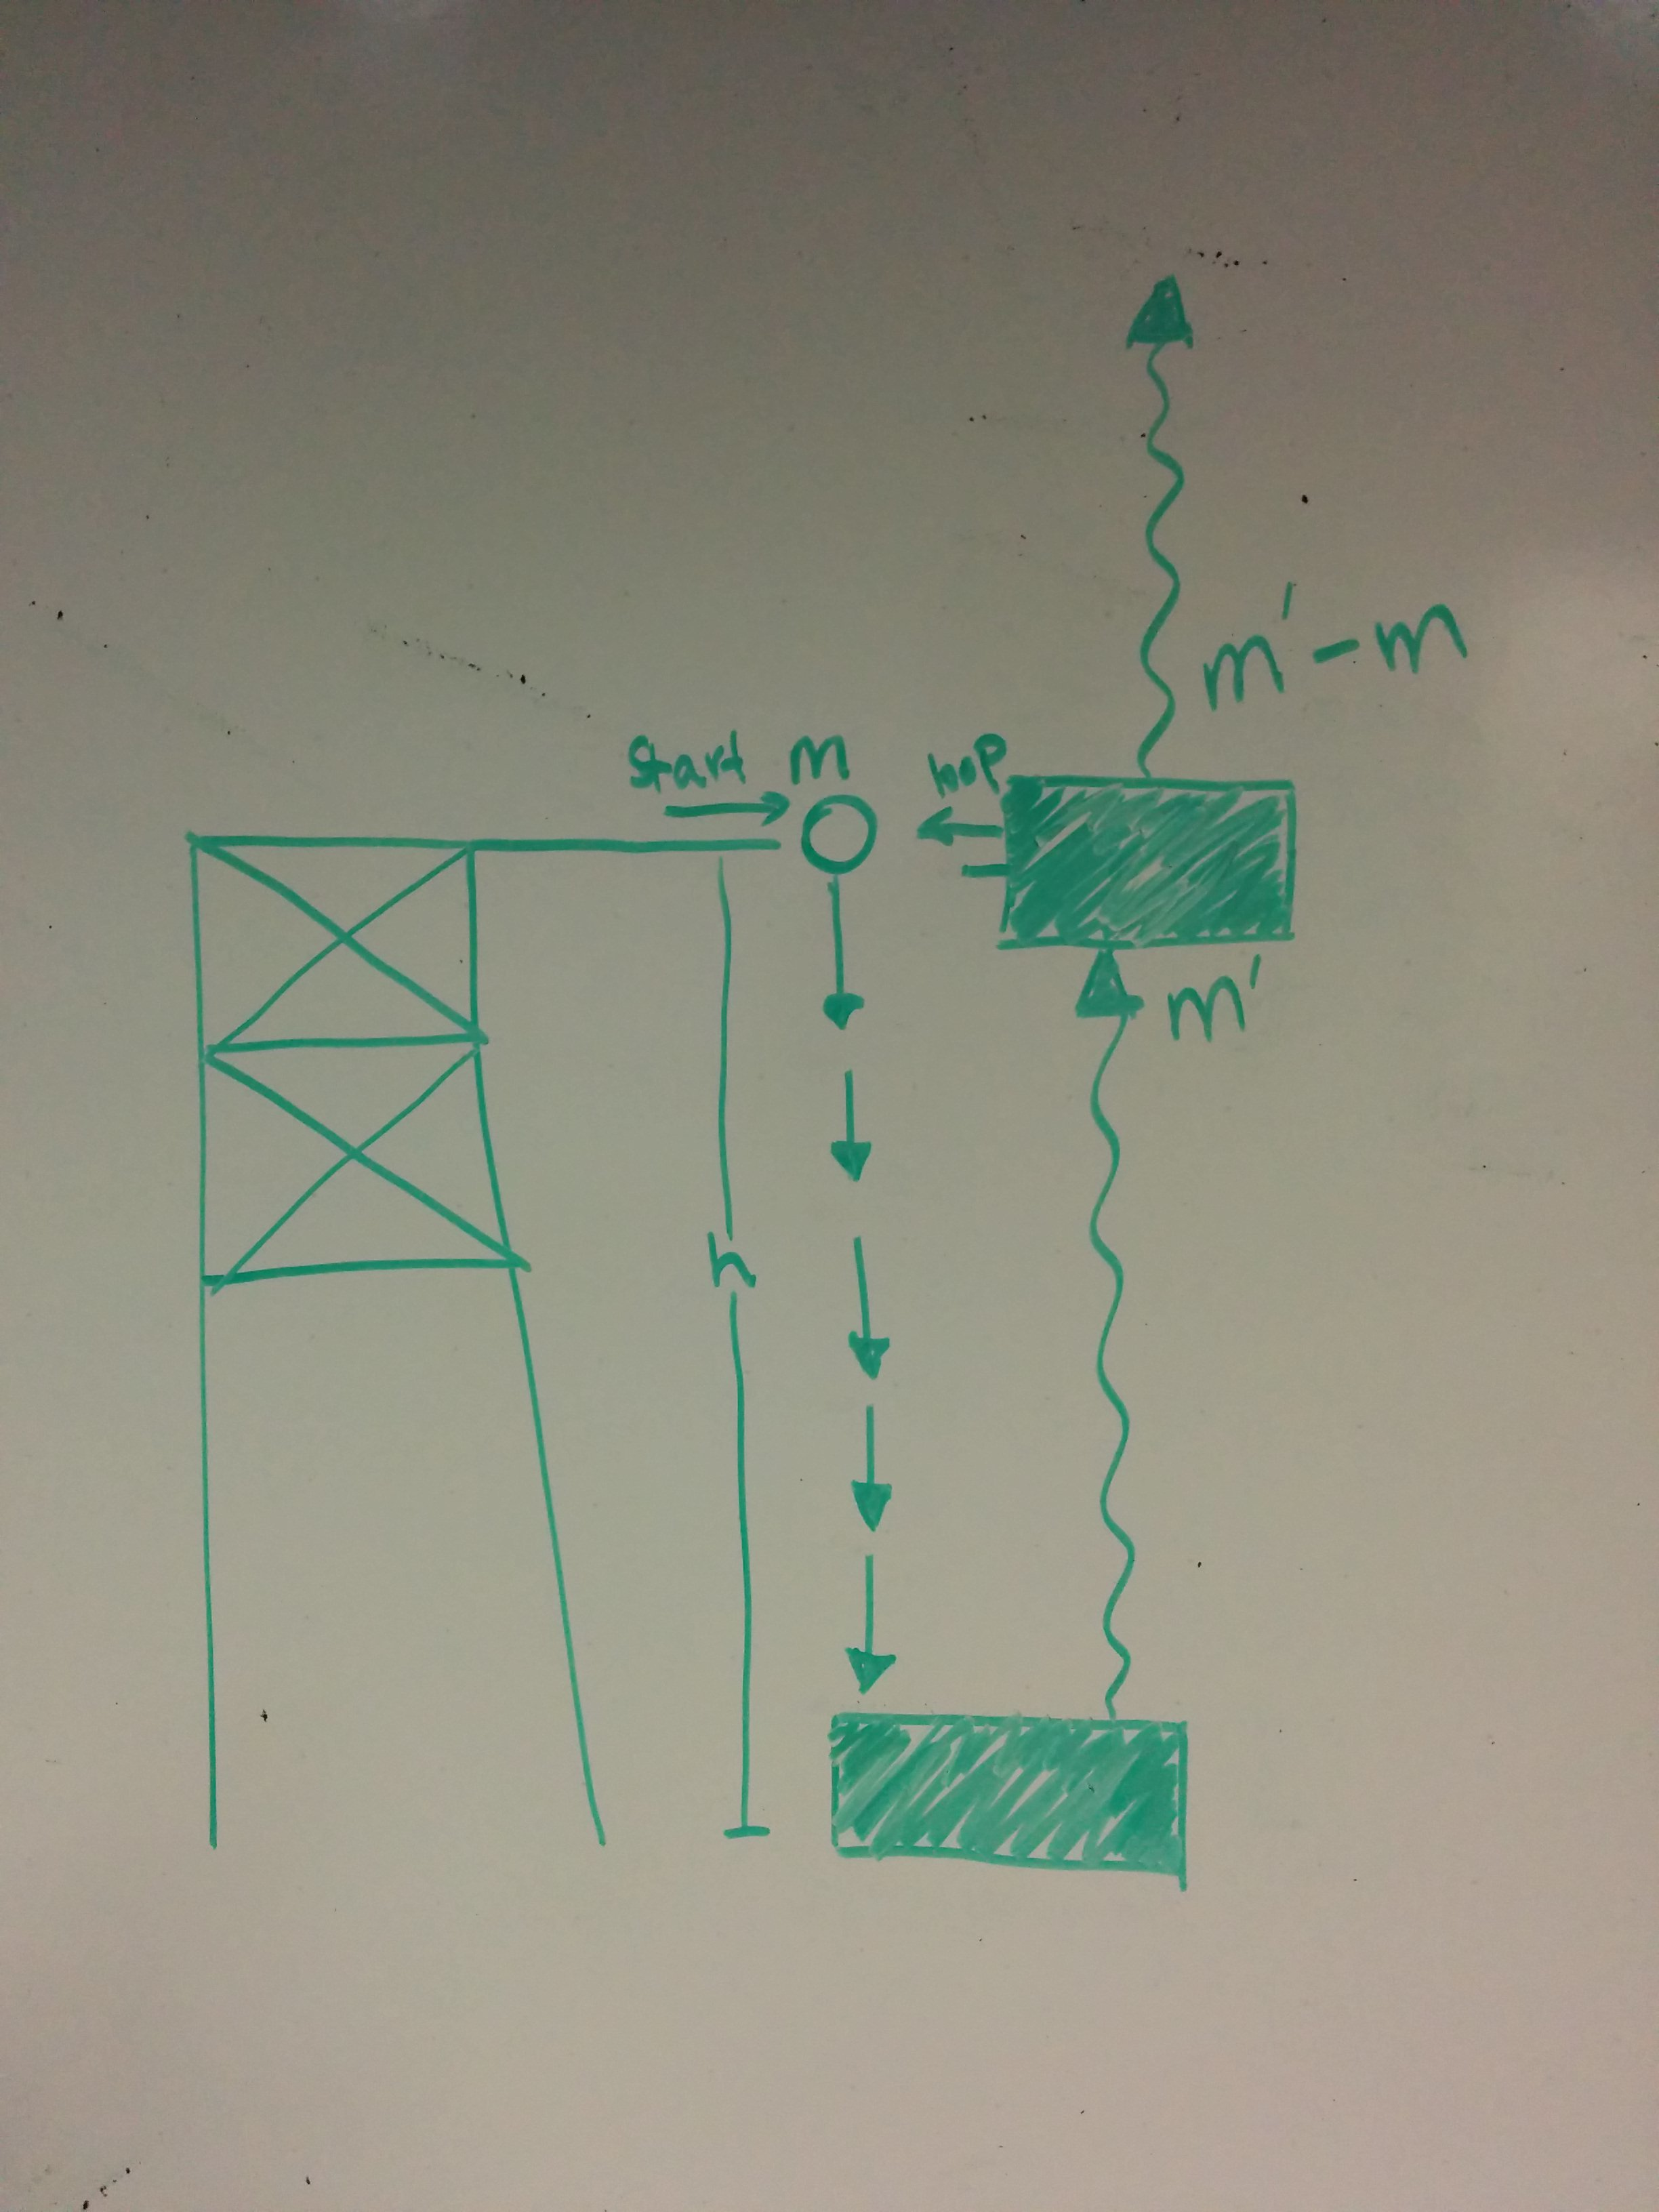
\includegraphics[width=0.75\textwidth]{img/ch5_problem_1b}
  \caption{Problem 1: Perpetual motion device.}
  \label{fig:ch5-problem-1b}
\end{figure}


\textbf{2}
Explain why a uniform gravitational field would not be able to create tides on Earth.

Tides depend on there being a gravitational field gradient. If the curvature closer to the source of the field (e.g. the Moon) is greater than it is further away, then the closer side will move towards the source more than the further side, thus creating tides. In the absense of such a gradient, there would be no difference in curvature between the two sides, and thus they would not stretch relative to each other.



\textbf{7}
Calculate the components of $\tensor{\Lambda}{^{\alpha'}_\beta}$ and $\tensor{\Lambda}{^\mu_{\nu'}}$ for transformations $(x, y) \leftrightarrow (r, \theta)$.
~
\begin{align*}
  \mqty( \Delta r \\ \Delta \theta ) &=
  \mqty( \pdv*{r}{x}      & \pdv*{r}{y} \\
         \pdv*{\theta}{x} & \pdv*{\theta}{y} )
  \mqty( \Delta x \\ \Delta y )
  &
  \mqty( \Delta x \\ \Delta y ) &=
  \mqty( \pdv*{x}{r} & \pdv*{x}{\theta} \\
         \pdv*{y}{r} & \pdv*{y}{\theta} )
  \mqty( \Delta r \\ \Delta \theta )
  \\ &=
  \mqty( x / \sqrt{x^2+y^2} & y / \sqrt{x^2 + y^2} \\
         -y / (x^2 + y^2) & x / (x^2 + y^2) )
  \mqty( \Delta x \\ \Delta y )
  &&=
  \mqty( \cos\theta & -r \sin\theta \\
         \sin\theta &  r \cos\theta )
  \mqty( \Delta r \\ \Delta \theta )
  \\ &=
  \mqty( \cos\theta & \sin\theta \\
         -(1/r) \sin\theta & (1/r) \cos\theta )
  \mqty( \Delta x \\ \Delta y )
  &&=
  \mqty( x / \sqrt{x^2 + y^2} & -y \\
         y / \sqrt{x^2 + y^2} &  x)
  \mqty( \Delta r \\ \Delta \theta )
\end{align*}
%
\begin{align*}
  \tensor{\Lambda}{^r_x} &= x / \sqrt{x^2 + y^2} = \cos\theta
  &
  \tensor{\Lambda}{^x_r} &= \cos\theta = x / \sqrt{x^2 + y^2}
  \\
  \tensor{\Lambda}{^r_y} &= y / \sqrt{x^2 + y^2} = \sin\theta
  &
  \tensor{\Lambda}{^y_r} &= -r \sin\theta = -y
  \\
  \tensor{\Lambda}{^\theta_x} &= -y / (x^2 + y^2) = -(1/r) \sin\theta
  &
  \tensor{\Lambda}{^x_\theta} &= \sin\theta = y / \sqrt{x^2 + y^2}
  \\
  \tensor{\Lambda}{^\theta_y} &= x / (x^2 + y^2) = (1/r) \cos\theta
  &
  \tensor{\Lambda}{^y_\theta} &= r \cos\theta = x
\end{align*}



\textbf{8}

(a)
$f \equiv x^2 + y^2 + 2xy$, $\vec{V} \underset{(x,y)}{\to} (x^2 + 3y, y^2 + 3x)$, $\vec{W} \underset{(r,\theta)}{\to} (1, 1)$. Express $f = f(r, \theta)$, and find the components of $\vec{V}$ and $\vec{W}$ in a polar basis, as functions of $r$ and $\theta$.

\begin{align*}
  f &= x^2 + y^2 + 2xy = (x + y)^2
  \\ &=
  (r \cos\theta + r \sin\theta)^2 =
  r^2 \sin^2\theta + r^2 \cos^2\theta + 2 r^2 \sin\theta \cos\theta
  \\ &=
  r^2 (1 + \sin(2 \theta))
  \\
%%%%%
  \vec{V} &\underset{(x,y)}{\to}
  \mqty( r^2 \cos^2\theta + 3 r \sin\theta \\
         r^2 \sin^2\theta + 3 r \cos\theta )
  \\
  \vec{V} &\underset{(r,\theta)}{\to}
  \mqty( \cos\theta & \sin\theta \\
         -(1/r) \sin\theta & (1/r) \cos\theta )
  \mqty( r^2 \cos^2\theta + 3 r \sin\theta \\
         r^2 \sin^2\theta + 3 r \cos\theta )
  \\ &\underset{(r,\theta)}{\to}
  \mqty(
    r^2 \cos^2\theta + 6 r \sin\theta \cos\theta + r^2 \sin^3\theta
    \\
    -r \cos^2\theta \sin\theta - 3 \sin^2\theta +
     r \sin^2\theta \cos\theta + 3 \cos^2\theta
  )
  \\ &\underset{(r,\theta)}{\to}
  \mqty(
    r^2 (\sin^3\theta + \cos^3\theta) + 6 r \sin\theta \cos\theta
    \\
    r \sin\theta \cos\theta (\sin\theta - \cos\theta) +
    3 (\cos^2\theta - \sin^2\theta)
  )
  \\ &\underset{(r,\theta)}{\to}
  \mqty(
    r^2 (\sin^3\theta + \cos^3\theta) + 3 r \sin(2\theta)
    \\
    (r/2) \sin(2\theta) (\sin\theta - \cos\theta) + 3 \cos(2\theta)
  )
  \\
%%%%%
  \vec{W} &\underset{(r,\theta)}{\to}
  \mqty( \cos\theta & \sin\theta \\
         -(1/r) \sin\theta & (1/r) \cos\theta )
  \mqty( 1 \\ 1 )
  \\ &\underset{(r,\theta)}{\to}
  \mqty(
    \cos\theta + \sin\theta
    \\
    (1/r) (\cos\theta - \sin\theta)
  )
\end{align*}



(b)
Express the components of $\tilde{\dd}f$ in $(x,y)$ and obtain them in $(r,\theta)$ by:

(i) using direct calculation in $(r, \theta)$:

\begin{displaymath}
  \tilde{\dd}f \underset{(r,\theta)}{\to}
  \qty( \pdv*{f}{r}, \pdv*{f}{\theta} ) =
  \qty( 2 r (1 + \sin(2 \theta)), 2 r^2 \cos(2 \theta) )
\end{displaymath}

(ii) transforming the components in $(x, y)$:

\begin{displaymath}
  \tilde{\dd}f \underset{(x,y)}{\to}
  \qty( \pdv*{f}{x}, \pdv*{f}{y} ) =
  \qty( 2 (x+y), 2 (x+y) ) =
  \qty( 2 r (\cos\theta + \sin\theta), 2 r (\cos\theta + \sin\theta))
\end{displaymath}

\begin{align*}
  \mqty( (\tilde{\dd}f)_r & (\tilde{\dd}f)_\theta ) &=
  \mqty( 1 & 1 )
  \mqty( \cos\theta & -r\sin\theta \\ \sin\theta & r\cos\theta )
  \qty[ 2 r (\cos\theta + \sin\theta) ]
  \\ &=
  \mqty( 2 r  (\cos^2\theta + \sin^2\theta + 2 \sin\theta\cos\theta) &
         2 r^2 (\cos^2\theta - \sin^2\theta) )
  \\ &=
  \mqty( 2 r (1 + \sin(2 \theta)) & 2 r^2 \cos(2 \theta) )
\end{align*}


(c)
Now find the $(r,\theta)$ components of the one-forms $\tilde{V}$ and $\tilde{W}$ associated with the vectors $\vec{V}$ and $\vec{W}$ by

(i)
using the metric tensor in $(r,\theta)$:


\begin{align*}
  V_r &=
  g_{r\alpha} V^\alpha =
  g_{rr} V^r + g_{r\theta} V^\theta
  \\ &=
  r^2 (\sin^3\theta + \cos^3\theta) + 3 r \sin(2\theta)
  \\
  V_\theta &=
  g_{\theta r} V^r + g_{\theta\theta} V^\theta =
  (1/2) r^3 \sin(2\theta) (\sin\theta - \cos\theta) +
  3 r^2 \cos(2\theta)
  \\
%%%%%
  W_r &=
  g_{r\alpha} W^\alpha =
  g_{rx} W^x + g_{ry} W^y
  \\ &=
  1 (\cos\theta + \sin\theta) +
  0 \qty[ (1/r) (\cos\theta - \sin\theta) ]
  \\ &=
  \cos\theta + \sin\theta
  \\
%%%%%
  W_\theta &=
  g_{\theta x} W^x + g_{\theta y} W^y =
  \\ &=
  0 (\cos\theta + \sin\theta) +
  r^2 \qty[ r (\cos\theta - \sin\theta) ]
  \\ &=
  r (\cos\theta - \sin\theta)
\end{align*}


(ii)
using the metric tensor in $(x,y)$ and then doing a coordinate transformation:

\begin{align*}
  V_x &= V^x; \quad V_y = V^y
  \\
  V_r &=
  \tensor{\Lambda}{^\alpha_r} V_\alpha =
  \tensor{\Lambda}{^x_r} V_x + \tensor{\Lambda}{^y_r} V_y
  \\ &=
  \cos\theta V_x + \sin\theta V_y
  \\ &=
  r^2 \cos^3\theta + (3/2) r \sin(2\theta) +
  r^2 \sin^3\theta + (3/2) r \sin(2\theta)
  \\ &=
  r^2 (\cos^3\theta + \sin^3\theta) + 3 r \sin(2\theta)
  \\
  V_\theta &=
  \tensor{\Lambda}{^\alpha_\theta} V_\alpha =
  \tensor{\Lambda}{^x_\theta} V_x + \tensor{\Lambda}{^y_\theta} V_y
  \\ &=
  (-r \sin\theta) V_x + (r \cos\theta) V_y
  \\ &=
  -r^3 \cos^2\theta \sin\theta - 3 r^2 \sin^2\theta +
   r^3 \sin^2\theta \cos\theta + 3 r^2 \cos^2\theta
  \\ &=
  r^3 \sin\theta \cos\theta (\sin\theta - \cos\theta) +
  3 r^2 (\cos^2\theta - \sin^2\theta)
  \\ &=
  (1/2) r^3 \sin(2\theta) (\sin\theta - \cos\theta) +
  3 r^2 \cos(2\theta)
  \\
%%%%%
  W_x &= W^x = W_y = W^y = 1
  \\
  W_r &=
  \tensor{\Lambda}{^\alpha_r} W_\alpha =
  \tensor{\Lambda}{^x_r} W_x + \tensor{\Lambda}{^y_r} W_y
  \\ &=
  \cos\theta + \sin\theta
  \\
  W_\theta &=
  \tensor{\Lambda}{^\alpha_\theta} W_\alpha =
  \tensor{\Lambda}{^x_\theta} W_x + \tensor{\Lambda}{^y_\theta} W_y
  \\ &=
  -r \sin\theta + r \cos\theta
  \\ &=
  r (\cos\theta - \sin\theta)
\end{align*}


\textbf{11}
Consider $V \underset{(x,y)}{\to} (x^2 + 3y, y^2 + 3x)$.

(a)
Find $\tensor{V}{^\alpha_{,\beta}}$ in Cartesian coordinates.
%
\begin{displaymath}
  \tensor{V}{^x_{,x}} = 2 x; \quad
  \tensor{V}{^y_{,y}} = 2 y; \quad
  \tensor{V}{^x_{,y}} = \tensor{V}{^y_{,x}} = 3.
\end{displaymath}

(b)
\begin{align*}
  \tensor{V}{^{\mu'}_{,\nu'}} &=
  \tensor{\Lambda}{^{\mu'}_\alpha}
  \tensor{\Lambda}{^\beta_{\nu'}}
  \tensor{V}{^\alpha_{,\beta}}
  \\
  \tensor{V}{^r_r} &=
  \tensor{\Lambda}{^r_x} \tensor{\Lambda}{^x_r} \tensor{V}{^x_{,x}} +
  \tensor{\Lambda}{^r_y} \tensor{\Lambda}{^y_r} \tensor{V}{^y_{,y}} +
  \tensor{\Lambda}{^r_x} \tensor{\Lambda}{^y_r} \tensor{V}{^x_{,y}} +
  \tensor{\Lambda}{^r_y} \tensor{\Lambda}{^x_r} \tensor{V}{^y_{,x}}
  \\ &=
  (\cos^2\theta) (2r \cos\theta) +
  (-r \sin^2\theta) (2r \sin\theta) +
  (-r \sin\theta \cos\theta) (3) +
  (\sin\theta \cos\theta) (3)
  \\ &=
  2r (\cos^3\theta - r \sin^3\theta) +
  \frac{3}{2} \sin(2\theta) (1 - r)
\end{align*}


(c)
\begin{align*}
  \tensor{V}{^{\mu'}_{;\nu'}} &=
  \tensor{V}{^{\mu'}_{,\nu'}}
  \tensor{V}{^{\alpha'}} \tensor{\Gamma}{^{\mu'}_{\alpha'\nu'}}
  \\
  \tensor{V}{^r_{;r}} &=
  \tensor{V}{^r_{,r}}
  \tensor{V}{^{\alpha'}} \tensor{\Gamma}{^{r}_{\alpha'r}}
  \\
  \tensor{V}{^\alpha} \tensor{\Gamma}{^r_{\alpha r}} &=
  V^r     \cancel{\tensor{\Gamma}{^r_{rr}}} +
  V^\theta \cancel{\tensor{\Gamma}{^r_{\theta r}}}
  \\
  \tensor{V}{^r_{;r}} &=
  \tensor{V}{^r_{,r}} =
  2r (\cos^3\theta - r \sin^3\theta) +
  \frac{3}{2} \sin(2\theta) (1 - r)
\end{align*}


(d)





(e)
\textbf{Requires parts (b) and (c) completed.}



\textbf{12}

\textbf{13}

\textbf{14}

\textbf{15}

\textbf{16}

\textbf{17}




\end{document}